\documentclass{beamer}
\usetheme{Madrid}
\colorlet{beamer@blendedblue}{green!40!black}
\setbeamertemplate{caption}[numbered]
\usepackage{amssymb, amsmath, amsthm}
\usepackage{physics, siunitx}
\usepackage{float, subcaption, graphicx}
\usepackage{hyperref}

\title{Lee Model}
\author{Hunt Feng\inst{1}}
\institute[Usask]
{
	\inst{1}%
	Department of Physics and Engineering Physics\\
	University of Saskatchewan
}
\date{\today}

%%%%%%%%%%%%%%%%%%%%
% section page 
%%%%%%%%%%%%%%%%%%%%
\AtBeginSection[]
{
	\begin{frame}{Outline of Presentation}
		\tableofcontents[currentsection]
	\end{frame}
}

\begin{document}
%%%%%%%%%%%%%%%%%%%%
% title and TOC
%%%%%%%%%%%%%%%%%%%%
\maketitle
\begin{frame}{Outline of Presentation}
    \tableofcontents
\end{frame}

%%%%%%%%%%%%%%%%%%%%
% contents 
%%%%%%%%%%%%%%%%%%%%
\section{Review of DPF}
\begin{frame} {Different Phases in DPF}
    \begin{itemize}
        \item Three phases: break down, axial, and compression phases.
        \item Compression phase: inward shockwave, reflected shockwave, and slow compression phase.
    \end{itemize}
\end{frame}

\begin{frame} {Break Down Phase}
    \begin{itemize}
        \item Gas is ionized, and current layer formed
    \end{itemize}
    \begin{figure}
        \centering
        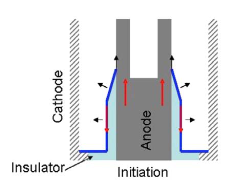
\includegraphics[width=0.5\textwidth]{figures/breakdown-phase.png}
        \caption{Initiation via flashover of the insulator. Break down phase. \cite{krishnan_2012_dense}}
        \label{fig:breakdown-phase}
    \end{figure}
\end{frame}

\begin{frame} {Axial Phase}
    \begin{itemize}
        \item Current layer is accelerated by the $\mathbf{J\times B}$ force in the axial direction.
        \item A shockwave (SW) is formed due to magnetic pressure (MP).
    \end{itemize}
    \begin{figure}
        \centering
        \begin{subfigure}{0.5\textwidth}
            \centering
            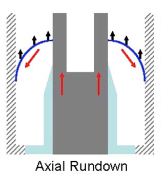
\includegraphics[width=0.5\textwidth]{figures/axial-rundown.png}
            \caption{Axial run-down phase. \cite{krishnan_2012_dense}}
        \end{subfigure}%
        \begin{subfigure}{0.5\textwidth}
            \centering
            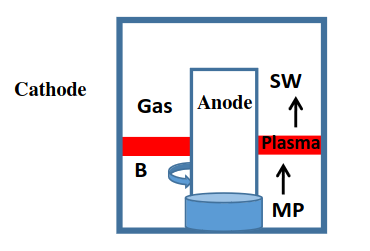
\includegraphics[width=0.7\textwidth]{figures/axial-phase.png}
            \caption{The formation of plasma layer. \cite{behbahani_2017_enhancement}}
        \end{subfigure}
        \label{fig:axial-phase}
    \end{figure}
\end{frame}

\begin{frame} {Compression Phase - Inward Shockwave Phase}
    \begin{itemize}
        \item When the plasma layer arrives at the top of the anode, the $\mathbf{J\times B}$ force pushes them into the center of the anode.
        \item Plasma column with inner radius $r_s$ and outer radius $r_p$ will form on the top of the anode.
        \item Shockwave compresses gas in the center.
    \end{itemize}
    \begin{figure}
        \centering
        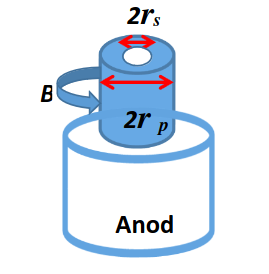
\includegraphics[width=0.4\textwidth]{figures/inward-shockwave-phase.png}
        \caption{The inward radial shock wave in final stage off plasma focus.}
        \label{fig:inward-shockwave-phase}
    \end{figure}
\end{frame}

\begin{frame} {Compression Phase - Reflected Shockwave Phase}
    \begin{itemize}
        \item The shockwave will be reflected radially in the outward direction after hitting the center of the anode.
    \end{itemize}
    \begin{figure}
        \centering
        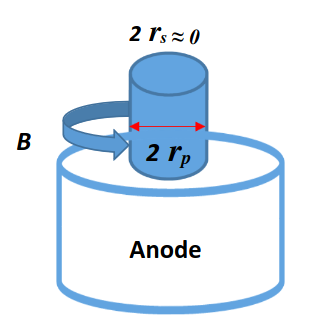
\includegraphics[width=0.4\textwidth]{figures/reflected-shockwave-phase.png}
        \caption{The reflected shockwave phase in plasma focus. \cite{behbahani_2017_enhancement}}
        \label{fig:reflected-shockwave-phase}
    \end{figure}
\end{frame}

\begin{frame} {Compression Phase - Slow Compression Phase}
    \begin{itemize}
        \item Slow compression phase starts when $r_s=r_p$.
        \item The reflected shockwave produces a pressure in the opposite direction of the magnetic pressure.
        \item Plasma column will be compressed to its minimum radius.
    \end{itemize}
\end{frame}

\begin{frame} {Instability Phase}
    \begin{itemize}
        \item When plasma reaches maximum compression, the plasma column may become unstable due to plasma instabilities.
        \item Instabilities make the plasma resistance anomalous.
    \end{itemize}
    \begin{figure}
        \centering
        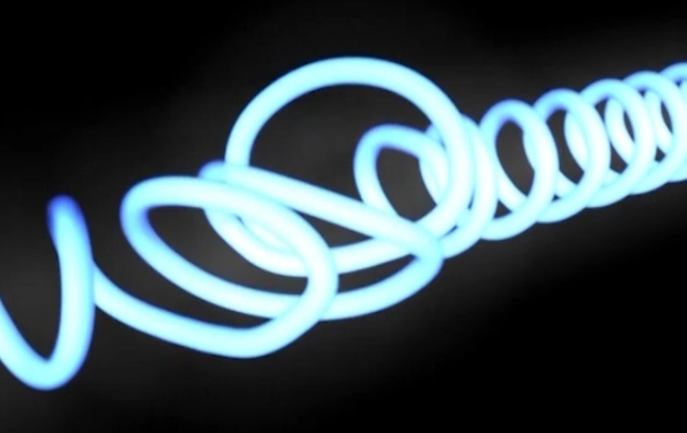
\includegraphics[width=0.7\textwidth]{figures/instability-phase.png}
        \caption{Plasma column is twisted in instability phase. Source \cite{lppfusion_device_fusion}}
        \label{fig:instability-phase}
    \end{figure}
\end{frame}
\section{Simulation}
\begin{frame} {Parameters}
    \begin{figure}
        \centering
        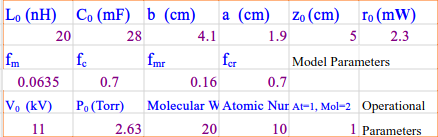
\includegraphics[width=0.7\textwidth]{figures/parameters.png}
        \caption{Input Parameters}
        \label{fig:parameters}
    \end{figure}
    \begin{itemize}
        \item The parameters are set to match the device NX2.
        \item Bank parameters, $L_0$, $C_0$ and stray circuit resistance $r_0$.
        \item Tube parameters $b$, $a$ and $z_0$.
        \item Operational parameters $V_0$ and $P_0$ and the fill gas.
    \end{itemize}
\end{frame}

\begin{frame} {Parameters - Continue}
    \begin{figure}
        \centering
        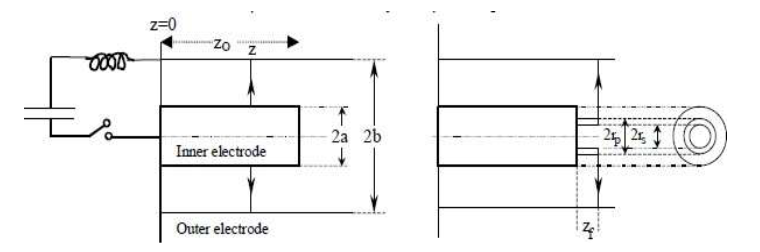
\includegraphics[width=\textwidth]{figures/dpf-device.png}
        \caption{DPF device.}
        \label{fig:dpf-device}
    \end{figure}
\end{frame}

\begin{frame} {Discharge Current}
    \begin{figure}
        \centering
        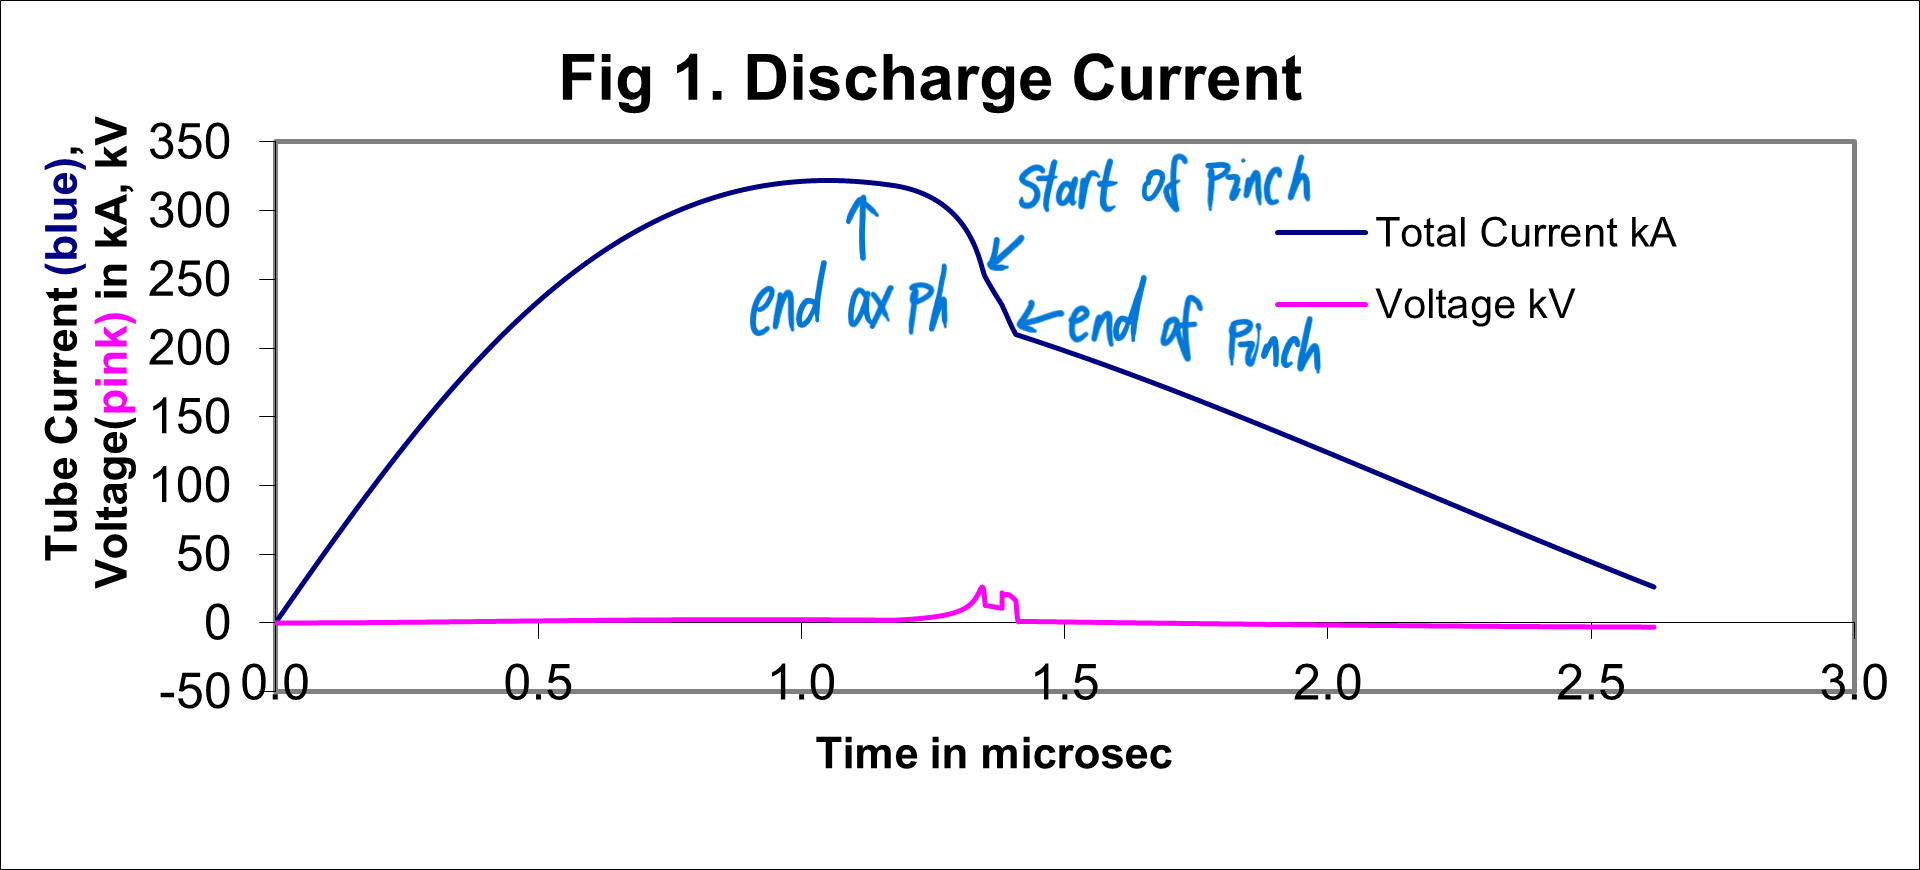
\includegraphics[width=0.7\textwidth]{figures/figure1.png}
        \caption{Discharge Current}
        \label{fig:discharge-Current}
    \end{figure}
    \begin{itemize}
        \item Axial phase ends after the discharge current reaches its peak (1.17\unit{\micro\s}).
        \item As the radial phase starts, the discharge current decreases.
        \item The pinch starts at 1.38\unit{\micro\s}.
        \item Then at 1.41\unit{\micro\s} the radial phase ends, also the pinch ends.
    \end{itemize}
\end{frame}

\begin{frame} {5-Point Fitting}
    \begin{figure}
        \centering
        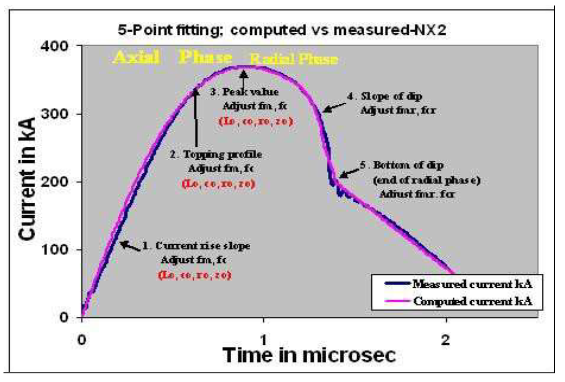
\includegraphics[width=0.5\textwidth]{figures/5-point-fitting.png}
        \caption{\scriptsize The 5-point fitting of computed current trace to measured (reference) current trace. Point 1 is the current rise slope. Point 2 is the topping profile. Point 3 is the peak value of the current. Point 4 is the slope of the current dip. Point 5 is the bottom of the current dip. Fitting is done up to point 5 only. Further agreement or divergence of the computed trace with/from the measured trace is only incidental and not considered to be important.}
        \label{fig:5-point-fitting}
    \end{figure}
    \begin{itemize}
        \item By fitting the 5 features, we are able to obtained the fitted model parameters: $f_m, f_c, f_{mr}$, and $f_{cr}$.
    \end{itemize}
\end{frame}

\begin{frame} {Speed of Current Sheet}
    \begin{figure}
        \centering
        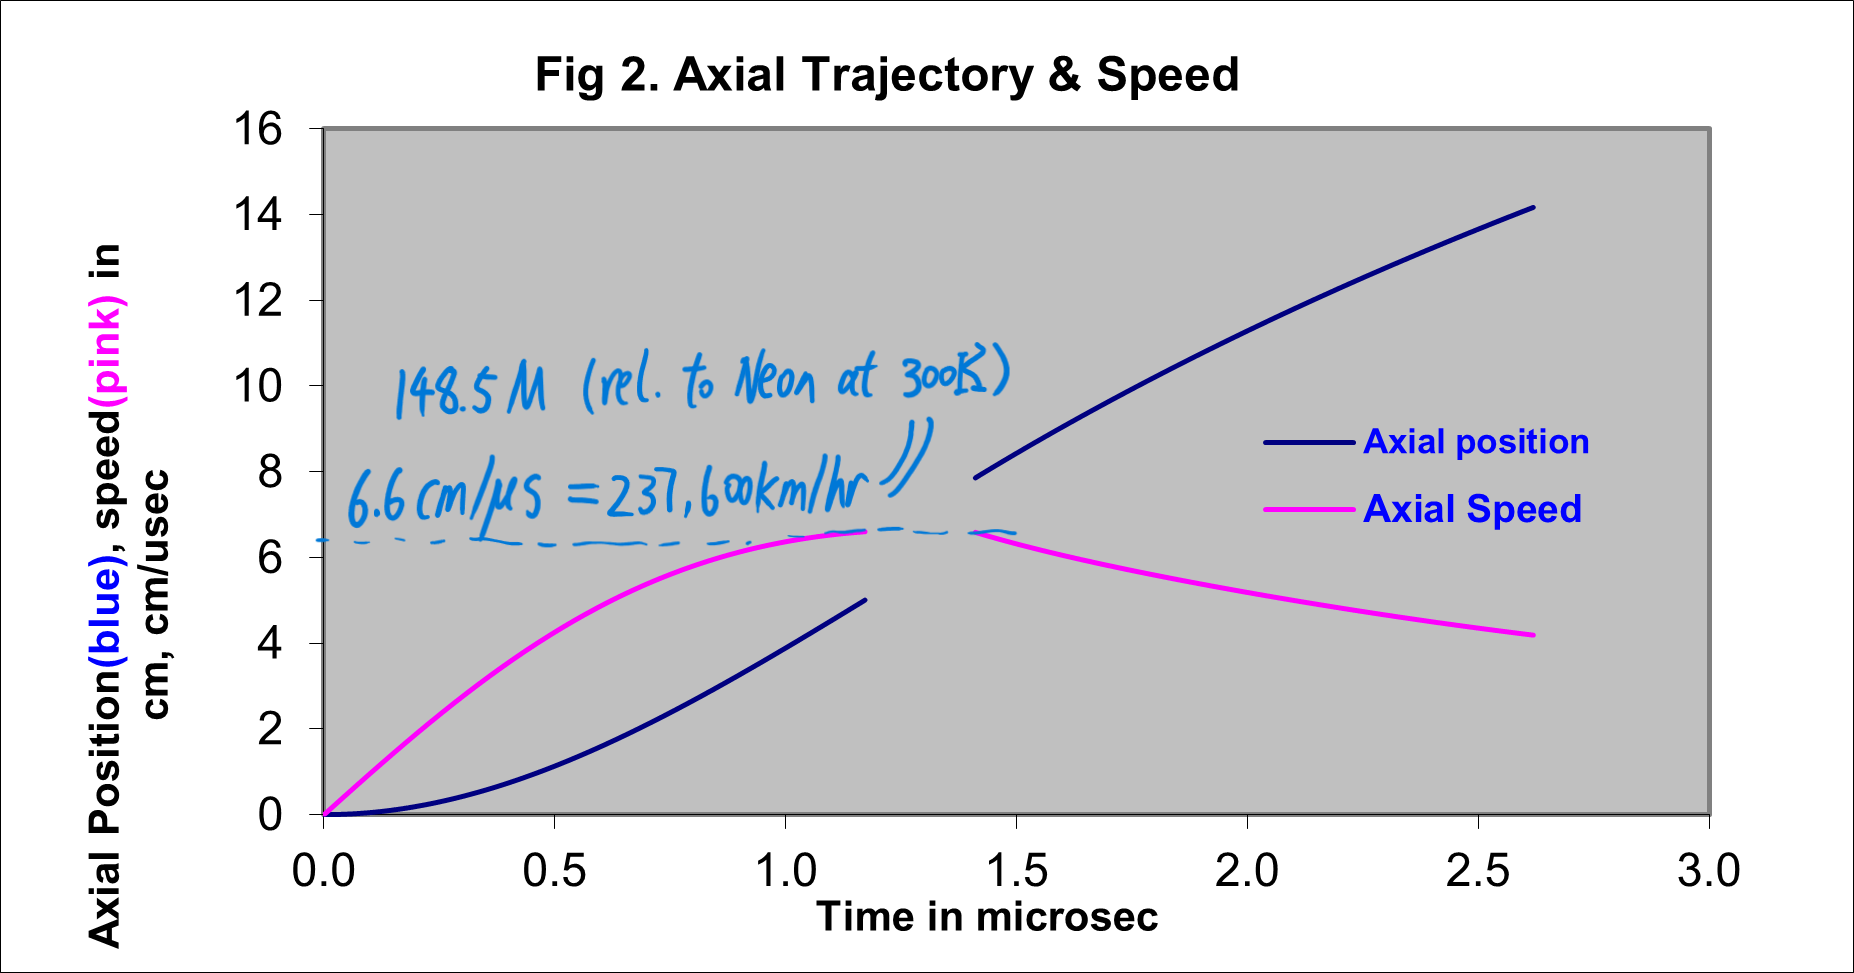
\includegraphics[width=0.7\textwidth]{figures/figure2.png}
        \caption{Axial Speed of the current sheet.}
        \label{fig:axial-speed}
    \end{figure}
    \begin{itemize}
        \item The speed of current sheet is fast.
        \item The speed of sound of Neon is 1500\unit{\kilo\m/\hour}. The Mach number is therefore 150M.
    \end{itemize}
\end{frame}

\begin{frame} {Radial Position}
    \begin{figure}
        \centering
        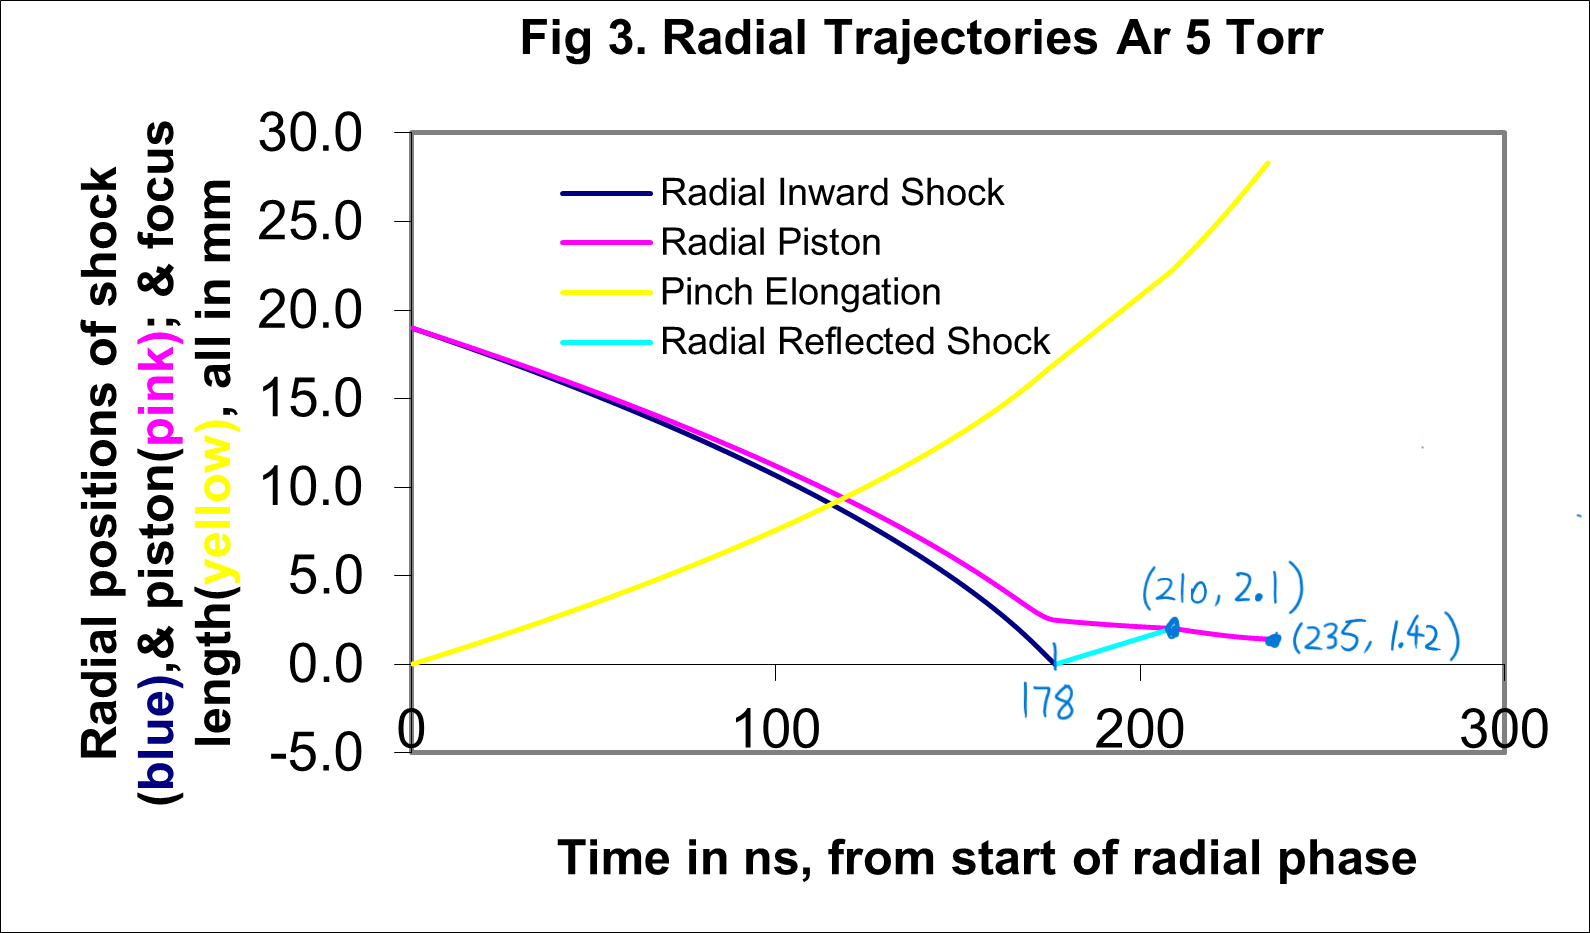
\includegraphics[width=0.55\textwidth]{figures/figure3.png}
        \caption{Radial position of the plasma column starting from radial phase.}
        \label{fig:radial-position}
    \end{figure}
    \begin{itemize}
        \item In the radial inward shock phase, both inner and outer radius of the plasma column decreases.
        \item After 178\unit{\nano\s}, radial reflected shock phase starts and the inner radius of the plasma column increases.
        \item After 210\unit{\nano\s}, it enters slow compression phase and the plasma column will be compressed to its minimum radius.
    \end{itemize}
\end{frame}

\begin{frame} {Temperature}
    \begin{figure}
        \centering
        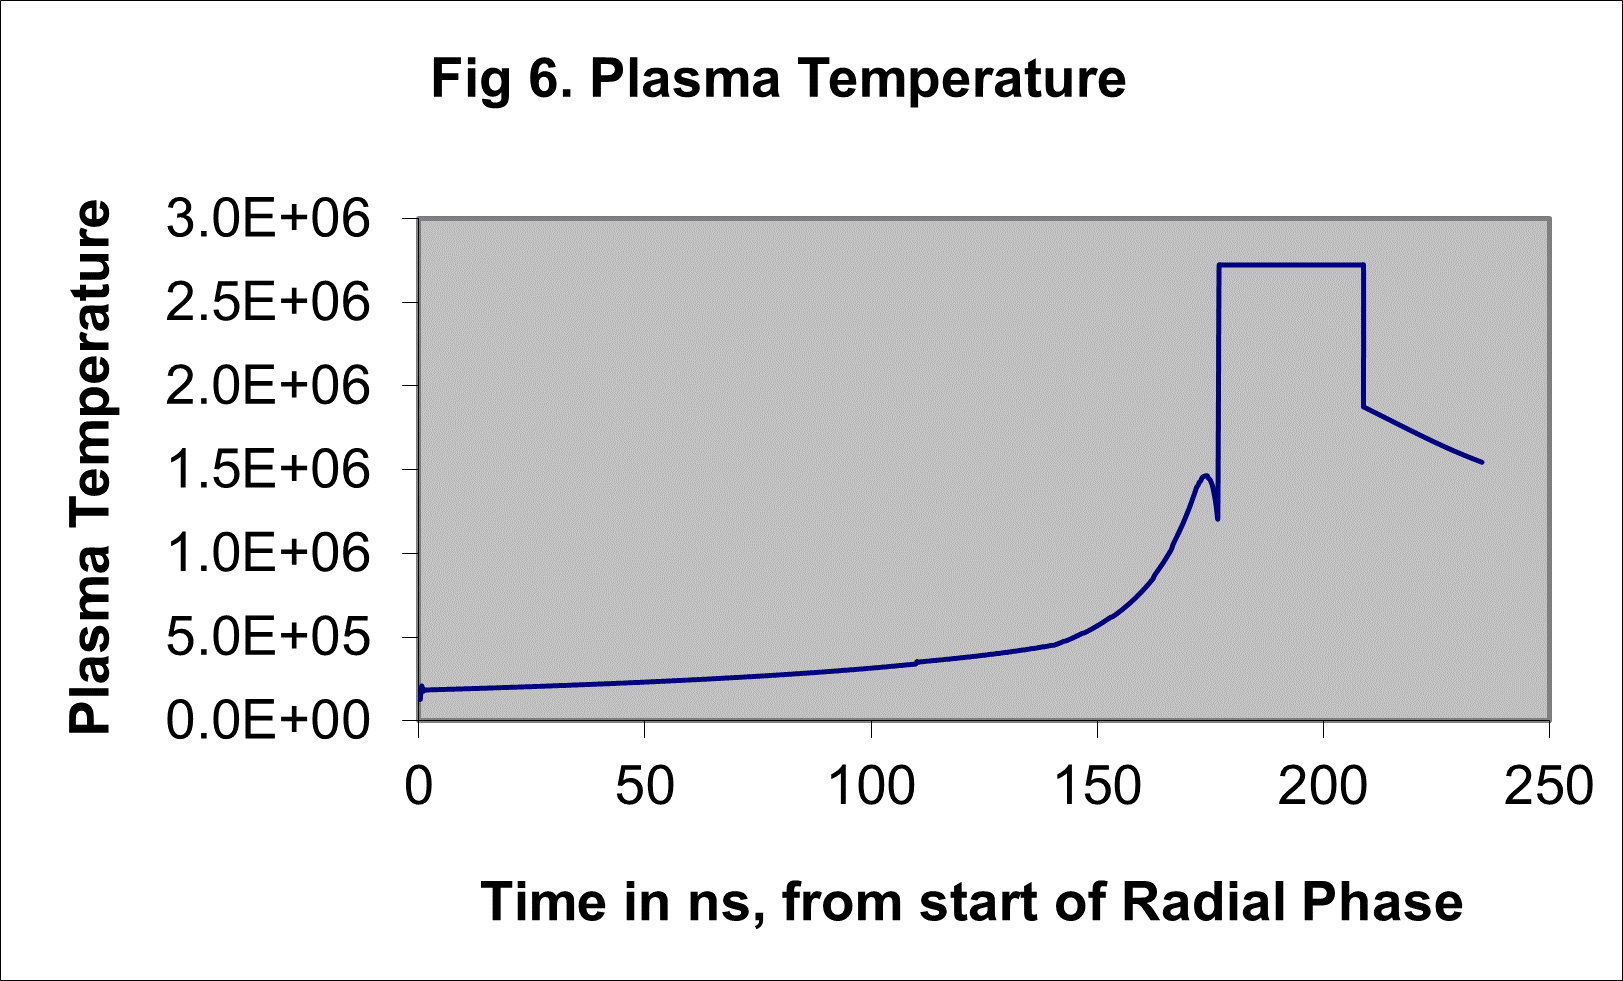
\includegraphics[width=0.6\textwidth]{figures/figure6.png}
        \caption{Plasma temperature in radial phase.}
        \label{fig:temperature}
    \end{figure}
    \begin{itemize}
        \item The plasma temperature raises during the radial inward shock phase.
        \item The plasma temperature reaches its maximum $2.72\times 10^6$K during the radial reflected shock phase.
        \item The temperature stays constant during the radial reflected shock phase.
    \end{itemize}
\end{frame}

\begin{frame} {Radiation}
    \begin{figure}
        \centering
        \begin{subfigure}{0.5\textwidth}
            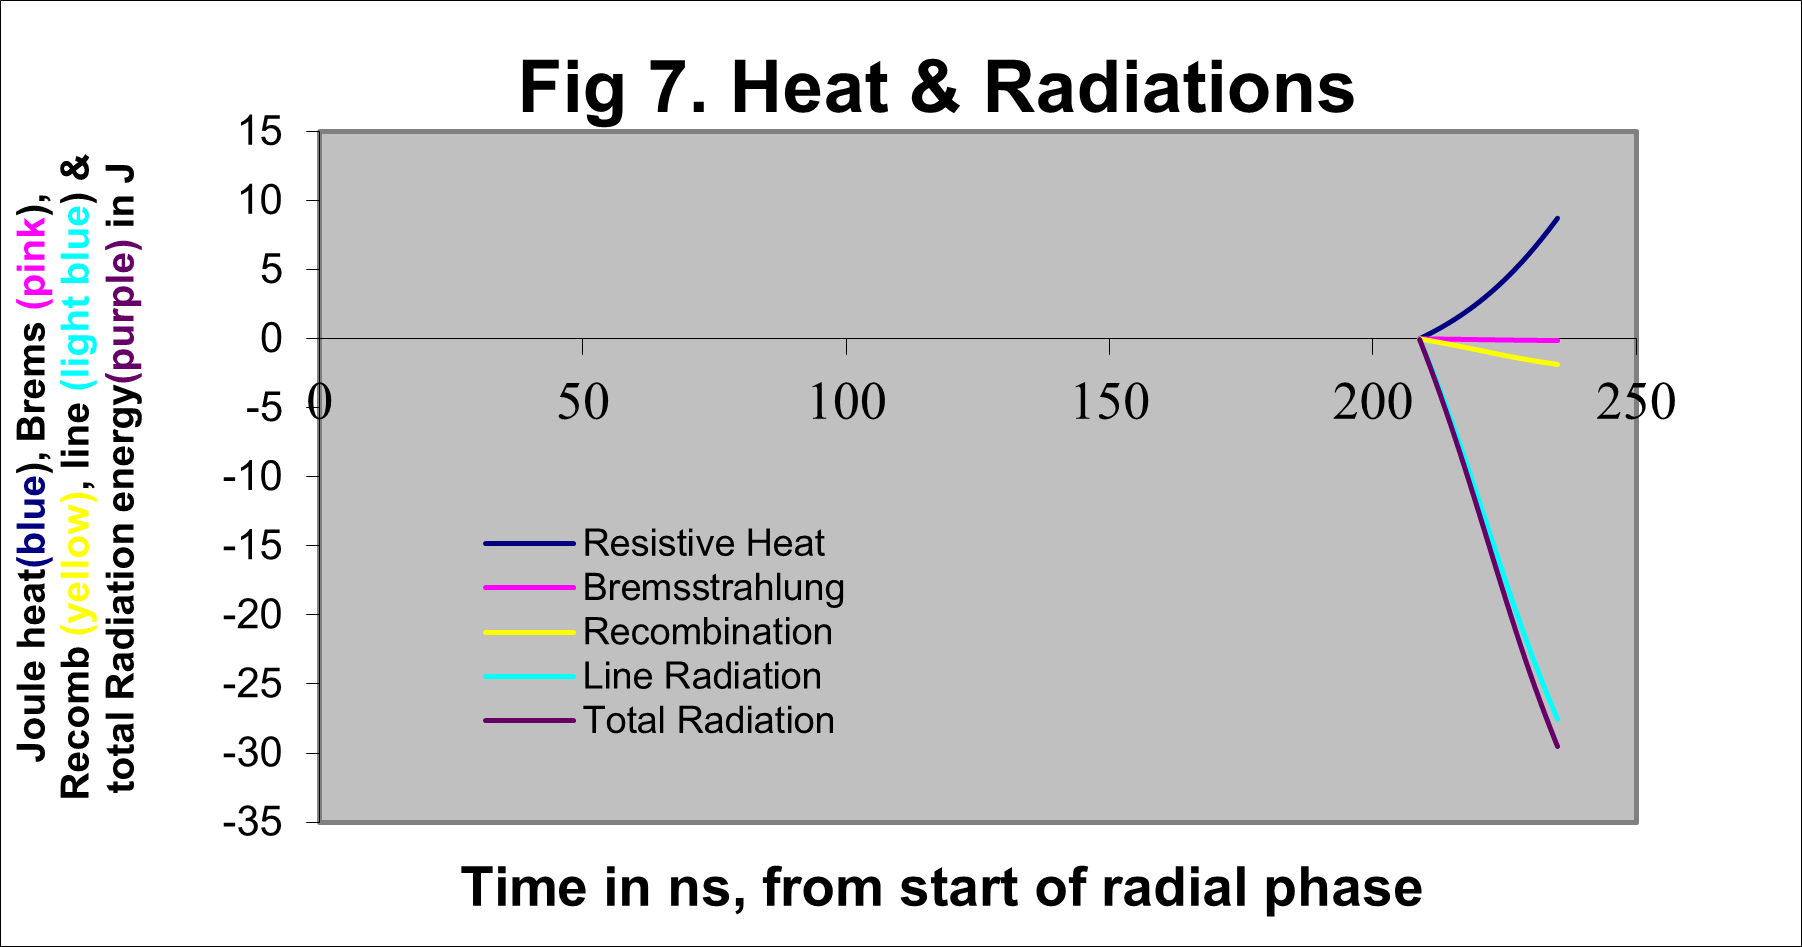
\includegraphics[width=\textwidth]{figures/figure7.png}
        \end{subfigure}%
        \begin{subfigure}{0.5\textwidth}
            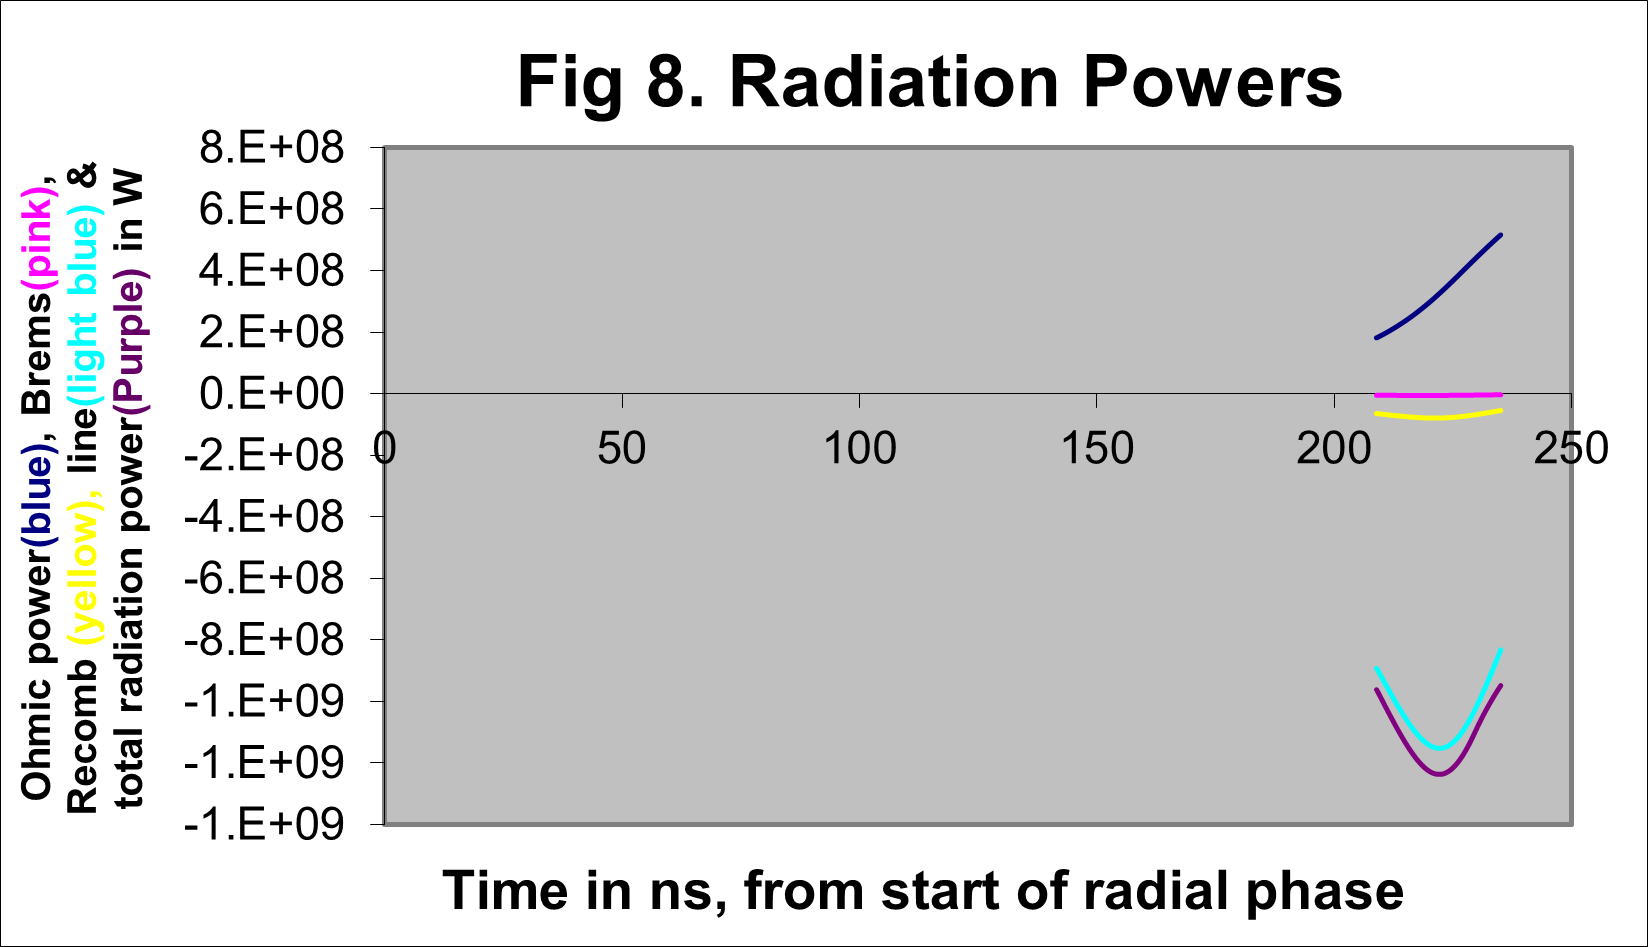
\includegraphics[width=0.9\textwidth]{figures/figure8.png}
        \end{subfigure}
        \caption{Radiation related graphs}
        \label{fig:radiation}
    \end{figure}
    \begin{itemize}
        \item Radiations starts after the pinch ends (plasmoid) is formed.
        \item Joule heating reached a maximum value of 8.73\unit{\J}
        \item Total radiation reached a maximum value of 30\unit{\J}
    \end{itemize}
\end{frame}

%%%%%%%%%%%%%%%%%%%%
% references
%%%%%%%%%%%%%%%%%%%%
\newpage
\begin{frame}[allowframebreaks]
    \bibliographystyle{abbrv}
    \bibliography{../references}
    \nocite{*}
\end{frame}

\end{document}